\documentclass[letterpaper]{article}

\usepackage{natbib,alifeconf}  %% The order is important
\usepackage{url,hyperref,cleveref}
\hypersetup{hidelinks,
  pdftitle={Survival Selection Grows a Private Kin Code, Not a Public Language},
  pdfauthor={Chunxuan Yang}}
\usepackage{booktabs}
\usepackage{placeins}

\newcommand\blfootnote[1]{%
  \begingroup
  \renewcommand\thefootnote{}\footnote{#1}%
  \addtocounter{footnote}{-1}%
  \endgroup
}

\title{Survival Selection Grows a Private Kin Code, Not a Public Language}
\author{
    Chunxuan Yang \\
    \mbox{}\\
    Sogang University, Seoul, Republic of Korea \\
    yang2023@sogang.ac.kr \quad yangchunxuan1@gmail.com
}

\begin{document}
\maketitle

\begin{abstract}
Can a decodable signalling code \emph{grow} from random weights under survival selection
alone, and is what grows public or private to kin? In a minimal hand-coded 2-D lethal-vent
world, tiny tied code-table agents evolve a decodable channel. Against an architecture-matched
random-fitness control (differing only in the reproduction-fitness signal), selection
\emph{sharpens} rather than originates it: clonal descent alone reaches mutual intelligibility
(MII) 0.1174 (${\sim}73\times$ the $1/625$ floor), and survival selection adds a paired
win-margin of $+0.0548$ (95\% CI $[0.0234, 0.0849]$, $n{=}48$) at gen 28, a margin a post-hoc
probe shows is a \emph{transient acceleration}. The code stays private to kin (dominant-lineage
share 99.1\%, $N_{\rm eff}$ 1.02): even under actively sustained diversity, and even when
survival is made to depend on decoding non-kin, no public cross-lineage code bootstraps, a
\emph{pressure-vs-survival tension}. We also contribute a bidirectional self-audit that catches
deflation as readily as inflation.
\end{abstract}

Submission type: \textbf{Late Breaking Abstracts}\\

Code \& verdict artifacts: \url{https://github.com/yangchunxuan/grown-grounded-language}; every result regenerates from committed, seeded verdict JSONs.\\
\blfootnote{\textcopyright{} 2026 Chunxuan Yang. Published under a Creative Commons Attribution 4.0 International (CC BY 4.0) license.}

\begin{figure*}[t!]
\centering
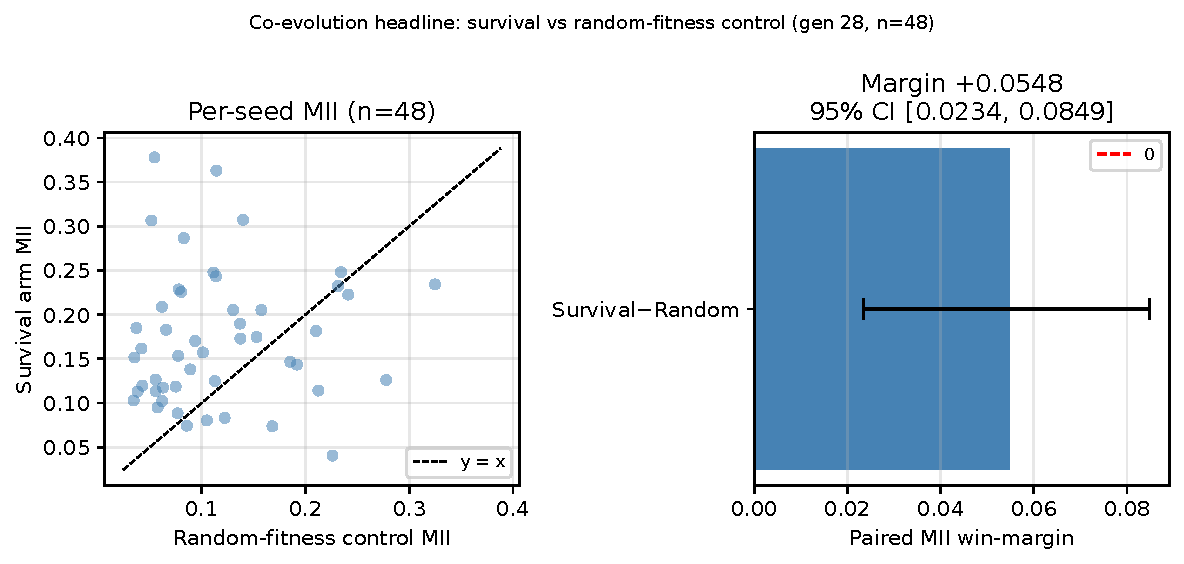
\includegraphics[height=3.5cm]{figs/f_headline.pdf}\hfill
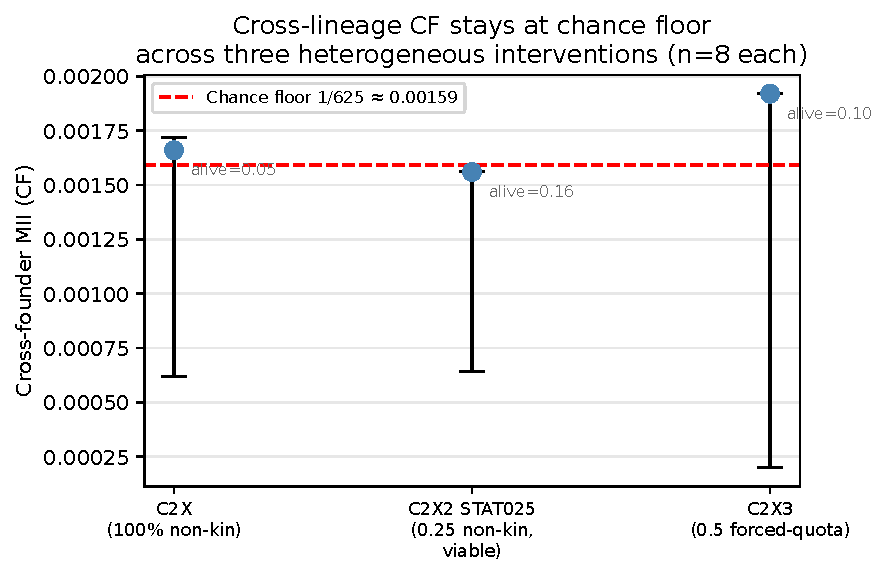
\includegraphics[height=3.5cm]{figs/f_crosslineage.pdf}
\caption{\textbf{A channel grows, but only kin can read it.} \textbf{(a)} Co-evolution headline
($n{=}48$, gen 28): the survival arm beats the architecture-matched random-fitness control by a
paired MII win-margin $+0.0548$ (95\% CI $[0.0234, 0.0849]$); a post-hoc probe shows this is a
transient acceleration. \textbf{(b)} Cross-founder MII stays at the chance floor
(${\approx}0.0016$) across three cross-lineage interventions ($n{=}8$); where pressure bites,
survival crashes. No public code bootstraps. Sources: committed verdict JSONs.}
\label{fig:main}
\end{figure*}

\section{The question and the world}
Where does a shared signalling code come from? Most computational accounts \emph{train} a
channel in (gradient descent on a task with a differentiable channel; \citealp{foerster2016,
lazaridou2017}) or \emph{design} one in (an imposed iterated-learning transmission bottleneck;
\citealp{kirby2008, ren2020}). We take up the prior question: can a decodable code \emph{grow}
from random weights under \textbf{survival selection alone}, and if it does, is it a
\textbf{public} code or a code private to \textbf{kin}?

The substrate is deliberately minimal and entirely hand-coded: a $48\times48$ lethal-vent
world in which agents metabolise, can die, and reproduce, and in which a single tied
\texttt{UnifiedIO} code-table ($4\times5\times6$, $\mathcal{N}(0,1)$ init) is the only
communicative apparatus. There is no gradient on communication, no oracle (agents never read
world truth), and no borrowed weights. We measure mutual intelligibility (MII) behaviourally:
route a referent through one agent's \texttt{emit} into another's \texttt{decode} and score
exact-tuple recovery against a chance floor of $1/625 \approx 0.0016$. Within-founder (WF) and
cross-founder (CF) MII separate a \emph{private kin code} (WF high, CF at chance) from a
\emph{public} one (CF also above chance).

\section{Co-evolution is real, but decomposes and stays kin-private}
The control is not communication-ablated: both arms carry the full code-table and run the
identical loop, and the only manipulated variable is the reproduction-fitness signal (survival
vs.\ uniform-random, with the reproduction RNG byte-matched). This isolates selection from
\emph{clonal descent-convergence}. The random-fitness arm also fixates to ${\sim}$one lineage,
so its MII of \textbf{0.1174} (${\sim}73\times$ floor) is the descent baseline, not zero. At
gen 28 the survival arm reaches \textbf{0.17219}, a paired win-margin of \textbf{$+0.0548$,
95\% CI $[0.0234, 0.0849]$} ($n{=}48$; \Cref{fig:main}, panel a). Selection therefore
\emph{sharpens} a largely descent-determined channel rather than originating it.

A post-hoc probe ($n{=}24$; gen 28/56/100/150) shows this is a \emph{transient acceleration}:
the survival-arm MII holds at ${\sim}0.16$--$0.17$ while the control's rises ($0.117 \to 0.138$)
as clonal fixation accumulates decodability, so the paired margin decays from $+0.0569$ (CI
excludes zero) to a CI including zero by gen 100. The headline is therefore scoped to 28
generations.

The code is \emph{not public}. The survival arm fixates to a single founder lineage
(dominant-lineage share \textbf{99.1\%}, $N_{\rm eff}$ \textbf{1.02}, 47/48 seeds
single-lineage), so WF runs ${\approx}0.16$ (${\sim}100\times$ chance) while CF sits at the
floor. Almost every receiver an agent meets is kin, so a private code is selectively cheap
\citep{hamilton1964}.

\section{The wall: no public code bootstraps}
Is kin-privacy merely an artifact of fast founder collapse? We sustained genuine multi-lineage
coexistence by niching (tournament selection plus lineage fitness-sharing) at pop=96: the
soft96 cell holds $N_{\rm eff}$ 4.10 over 20+ coexisting generations, yet CF stays at the floor
(CF $0.00153$ vs.\ floor $0.0016$; the CF$-$floor CI straddles zero). Maintaining diversity is
\emph{necessary but not sufficient}.

Making survival itself depend on decoding non-kin does not help either. Across three
heterogeneous interventions (\Cref{fig:main}, panel b: C2X2 at 0.25 non-kin stays viable
(alive 0.16) yet CF 0.00156; C2X3 at 0.5 non-kin alive 0.10, CF 0.00192; C2X at 100\% non-kin
crashes to alive 0.046), CF never rose above chance; where the pressure bit, it crashed
survival. Non-kin codes are mutually undecodable, so forced cross-listening is
acting on noise, which starves foraging: a \emph{pressure-vs-survival tension}. All
cross-lineage arms are $n{=}8$ (positive-or-inconclusive tier), so we report that a public code
\emph{did not} bootstrap under the regimes tested, never that none \emph{can}.

% Cross-lineage interventions are shown visually in Figure~\ref{fig:main}(b); per-cell numbers are in-text below.

\section{A bidirectional self-audit}
Each claim must survive an architecture-matched control, a fair baseline, $\geq$6-seed
bootstrap-CI win-margins, frozen pre-registration, a no-oracle redline, and code-grounded
adversarial review. Its single methodological claim is \emph{bidirectionality}: it catches
deflation as readily as inflation. Two in-scope catches show this: a pilot/formal false
\emph{negative} (a formal arm compared against a pilot control had buried a real effect, with
generation count the load-bearing knob), and an RNG-offset bug in the headline control whose
fix left the conclusion intact and slightly \emph{strengthened} the margin
($+0.045 \to +0.0548$).

\section{Contribution and scope}
This separates three claims often conflated in emergent-language work: a decodable code can
\emph{evolve}, it can \emph{matter} for survival, and it can still \emph{fail to become
public}. A decodable code grows from scratch under survival selection but stays kin-private;
selection \emph{accelerates} a clonal-descent channel rather than originating a public one; and
no public code bootstraps even under sustained diversity and direct cross-lineage pressure. The results
are scoped to one hand-coded world, one architecture, and per-stage timescales (28--48
generations). We read the wall as motivating a richer world and a consequence-driven learner
rather than more selection pressure. All code and seeded verdict JSONs are committed and
reproducible.

\FloatBarrier
\footnotesize
\begin{thebibliography}{9}
\setlength{\itemsep}{0pt}
\bibitem[Foerster et al.(2016)]{foerster2016} Foerster, J., et al. (2016). Learning to communicate with deep multi-agent reinforcement learning. \emph{NeurIPS}.
\bibitem[Hamilton(1964)]{hamilton1964} Hamilton, W. D. (1964). The genetical evolution of social behaviour. \emph{J. Theor. Biol.}, 7(1).
\bibitem[Kirby et al.(2008)]{kirby2008} Kirby, S., Cornish, H., and Smith, K. (2008). Cumulative cultural evolution in the laboratory. \emph{PNAS}, 105(31).
\bibitem[Lazaridou et al.(2017)]{lazaridou2017} Lazaridou, A., Peysakhovich, A., and Baroni, M. (2017). Multi-agent cooperation and the emergence of (natural) language. \emph{ICLR}.
\bibitem[Ren et al.(2020)]{ren2020} Ren, Y., et al. (2020). Compositional languages emerge in a neural iterated learning model. \emph{ICLR}.
\end{thebibliography}

\end{document}
